% !TeX spellcheck = en_US
%\documentclass[11pt,a4paper]{article}
\documentclass[11pt
  , a4paper
  , article
  , oneside
%  , twoside
%  , draft
]{memoir}

\usepackage{control}
\usepackage{kotex}
\usepackage[numbers]{natbib}
%\usepackage[pdftex]{graphicx}
%\DeclareGraphicsExtensions{.pdf,.png,.jpg}
\begin{document}

\newcommand{\technumber}{
  Digital Signal Processing using MATLAB\\
  Document 1: 2016-03-26}
\title{\textbf{Digital Signal Processing: 실습 7 \\
		제4장 z-변환 \\}}

\author{이상일\thanks{silee7103@ibs.re.kr} \\

  학번: 201460437\\
  Computer Engineering, Chungnam National University 
}
\date{\today}

\renewcommand{\maketitlehooka}{\begin{flushright}\textsf{\technumber}\end{flushright}}
%\renewcommand{\maketitlehookb}{\centering\textsf{\subtitle}}
%\renewcommand{\maketitlehookc}{C}
%\renewcommand{\maketitlehookd}{D}

\maketitle

\begin{abstract}
MATLAB을 사용한 Digital Signal Processing에 대한 실습과제에 대한 Documents를 구성한다.
\end{abstract}

\chapter{Example 4-4:}

\begin{lstlisting}[style=termstyle]
Example 4.4

x1 =[2,3,4]; x2=[3,4,5,6]; x3 = conv(x1,x2)
\end{lstlisting}

\begin{figure}[h!]
	\centering
	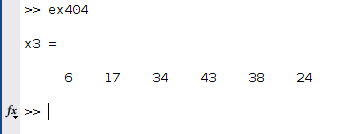
\includegraphics[width=0.3\textwidth,height=0.15\textwidth]{./images/ex404.png}
	\caption{Example 4.4 Result}
	\label{fig:Example 4.4 Result}
\end{figure}

\chapter{Example 4-5:}
\begin{lstlisting}[style=termstyle]
%Example 4.5

x1 =[1,2,3]; n1=[-1:1]; x2=[2,3,4,5]; n2=[-2:1];
[x3, n3] =  conv_m(x1,n1,x2,n2)
\end{lstlisting}

\clearpage

\begin{figure}[h!]
	\centering
	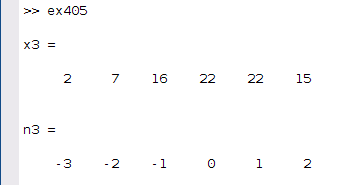
\includegraphics[width=0.3\textwidth,height=0.15\textwidth]{./images/ex405.png}
	\caption{Example 4.5 Result}
	\label{fig:Example 4.5 Result}
\end{figure}

\chapter{Example 4-6:}
\begin{lstlisting}[style=termstyle]
%Example 4.6

b = [0,0,0,0.25,-0.5,0.0625];
a = [1,-1,0.75,-0.25,0.0625];

[delta, n]=impseq(0,0,7) 

x = filter(b,a,delta)

x = [(n-2).*(1/2).^(n-2).*cos(pi*(n-2)/3)].*stepseq(2,0,7)
\end{lstlisting}

\begin{figure}[h!]
	\centering
	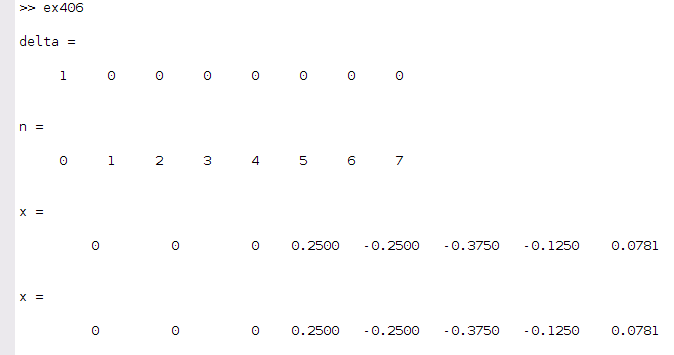
\includegraphics[width=0.3\textwidth,height=0.15\textwidth]{./images/ex406.png}
	\caption{Example 4.6 Result}
	\label{fig:Example 4.6 Result}
\end{figure}

\chapter{Example 4-8:}
\begin{lstlisting}[style=termstyle]
%Example 4.8

b = [0,1]; a = [3,-4,1]; [R,p,C ] = residuez(b,a)
[b, a] = residuez(R,p,C)
\end{lstlisting}

\begin{figure}[h!]
	\centering
	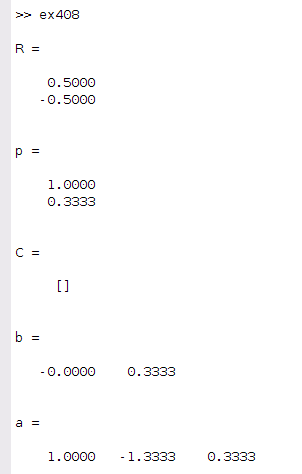
\includegraphics[width=0.3\textwidth,height=0.15\textwidth]{./images/ex408.png}
	\caption{Example 4.8 Result}
	\label{fig:Example 4.8 Result}
\end{figure}

\clearpage

\chapter{Example 4-9:}
\begin{lstlisting}[style=termstyle]
%Example 4.9

b = 1; a = poly([0.9,0.9,-0.9])
[R,p,C ] = residuez(b,a)

[delta, n]=impseq(0,0,7); 

x = filter(b,a,delta)
x = (0.75)*(0.9).^n + (0.5)*n.*(0.9).^n + (0.25)*(-0.9).^n
\end{lstlisting}

\begin{figure}[h!]
	\centering
	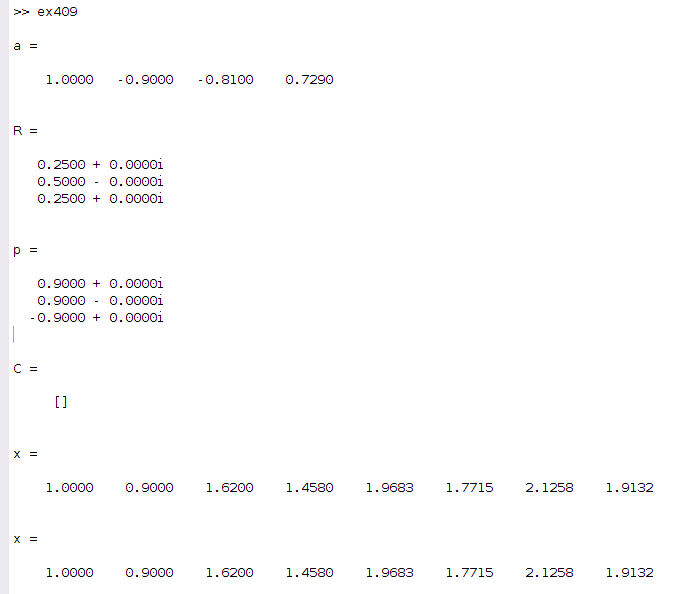
\includegraphics[width=0.3\textwidth,height=0.15\textwidth]{./images/ex409.png}
	\caption{Example 4.9 Result}
	\label{fig:Example 4.9 Result}
\end{figure}

\chapter{연습문제 4.1: }
\section{4.1-1: }
\begin{lstlisting}[style=termstyle]
n1 = [0:3]; y1 = [1 -2 3 -4]; n2 = [0:3]; y2 = [4 3 -2 1];
[x1,n] = conv_m(y1,n1,y2,n2)
\end{lstlisting}

\begin{figure}[h!]
	\centering
	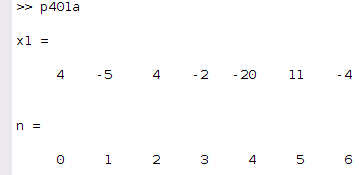
\includegraphics[width=0.3\textwidth,height=0.15\textwidth]{./images/p401-1.png}
	\caption{Problem 4.1-1 Result}
	\label{fig:Problem 4.1-1 Result}
\end{figure}
따라서, 
\begin {equation}
X1(z) = 4 -5z^{-1}+4z^{-2}-2z^{-3}-20z^{-4}+11z^{-5}-4z^{-6}
\end {equation}

\clearpage
\section{4.1-2: }
\begin{lstlisting}[style=termstyle]
n1 = [-2:2]; y1 = [1 -2 3 2 1]; n2 = [-3:3]; y2 = [1 0 0 0 0 0 1];
[x2,n] = conv_m(y1,n1,y2,n2)
\end{lstlisting}

\begin{figure}[h!]
	\centering
	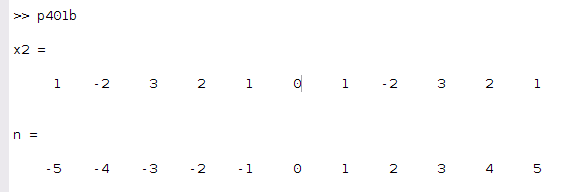
\includegraphics[width=0.3\textwidth,height=0.15\textwidth]{./images/p401-2.png}
	\caption{Problem 4.1-2 Result}
	\label{fig:Problem 4.1-2 Result}
\end{figure}
따라서, 
\begin {equation}
X2(z)=z^{5} - 2z^{4} + 3z^{3} + 2z^{4} + z + z^{-1} -2z^{-2} + 3z^{-3} + 2z^{-4}+ z^{-5}
\end {equation}
\section{4.1-3: }
\begin{lstlisting}[style=termstyle]
n1 = [0 1 2]; y1 = [1 1 1]; [y2,n2] = conv_m(y1,n1,y1,n1);
[x3,n] = conv_m(y1,n1,y2,n2)
\end{lstlisting}

\begin{figure}[h!]
	\centering
	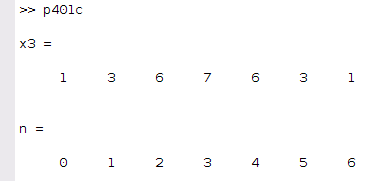
\includegraphics[width=0.3\textwidth,height=0.15\textwidth]{./images/p401-3.png}
	\caption{Problem 4.1-3 Result}
	\label{fig:Problem 4.1-3 Result}
\end{figure}
따라서, 
\begin {equation}
X3(z)= 1 + 3z^{-1} + 6z^{-2} + 7z^{-3} + 6z^{-4} + 3z^{-5} + z^{-6}
\end {equation}
\clearpage
\section{4.1-4: }
\begin{lstlisting}[style=termstyle]
n11 = [0:3]; y11 = [1 -2 3 -4]; n12 = [0:3]; y12 = [4 3 -2 1];
[y13,n13] = conv_m(y11,n11,y12,n12);
n21 = [-2:2]; y21 = [1 -2 3 2 1]; n22 = [-3:3]; y22 = [1 0 0 0 0 0 1];
[y23,n23] = conv_m(y21,n21,y22,n22);
n31 = [0 1 2]; y31 = [1 1 1];
[y32,n32] = conv_m(y31,n31,y31,n31); [y33,n33] = conv_m(y31,n31,y32,n32);
[y41,n41] = conv_m(y13,n13,y23,n23); [x4,n] = sigadd(y41,n41,y33,n33)
\end{lstlisting}

\begin{figure}[h!]
	\centering
	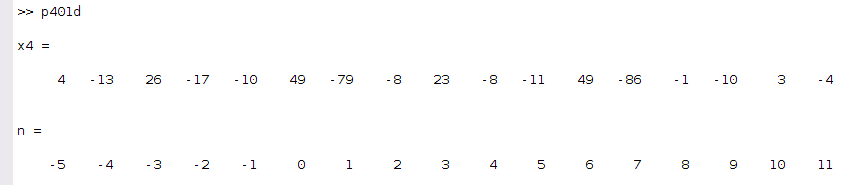
\includegraphics[width=0.3\textwidth,height=0.15\textwidth]{./images/p401-4.png}
	\caption{Problem 4.1-4 Result}
	\label{fig:Problem 4.1-4 Result}
\end{figure}

따라서, 
\begin {equation}
\begin {split}
X4(z)= 4z^5 - 13z^4 + 26z^3 - 17z^2 -10z^1 + 49 -79z^{-1} - 8z^{-2} +23z^{-3} - 8z^{-4} -11z^{-5}  &+\\ 49z^{-6} -86z^{-7} -z^{-8} -10z^{-9} +3z^{-10} -4z^{-11}
\end{split}
\end {equation}

\section{4.1-5: }
\begin{lstlisting}[style=termstyle]
n1 = [0:9]; y1 = [0 1 0 -3 0 2 0 5 0 -1]; n2 = [-4:0]; y2 = [4 2 3 1 0];
[x5,n] = conv_m(y1,n1,y2,n2)
\end{lstlisting}

\begin{figure}[h!]
	\centering
	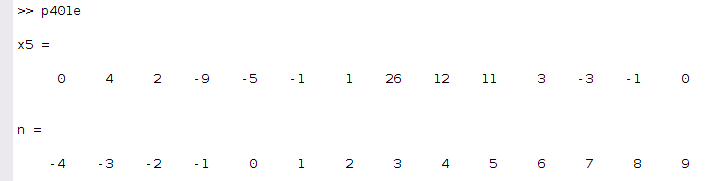
\includegraphics[width=0.3\textwidth,height=0.15\textwidth]{./images/p401-5.png}
	\caption{Problem 4.1-5 Result}
	\label{fig:Problem 4.1-5 Result}
\end{figure}
따라서, 
\begin {equation}
X5(z)= 4z^3 + 2z^2 - 9z^1 -5 -z^{-1} + z^{-2} +26z^{-3}+12z^{-4}+11z^{-5}+3z^{-6}-3z^{-7}-z^{-8}
\end {equation}

\clearpage

\chapter{연습문제 4.5: }
\section{4.5-1: }

z-transform:
\begin {equation}
X(z)= 2z^{-2} + 3z^{-3}\frac{1}{1-z^{-1}} = \frac{2z^{-2}+z^{-3}}{1-z^{-1}}, |z| > 1
\end {equation}


\begin{lstlisting}[style=termstyle]
b = [0 -8 0 -1.5 0 -1/16]; a = [1 0 3/16 0 3/256 0 1/(256*16)];
[delta,n1] = impseq(0,0,9); xb1 = filter(b,a,delta);
[u,n2] = stepseq(0,0,9);xb2 = (((n2-3).*((1/4).^(n2-2))).*cos((pi/2)*(n2-1))).*u;
error = max(abs(xb1-xb2))
[Hz,Hp,Hl] = zplane(b,a); set(Hz,'linewidth',1); set(Hp,'linewidth',1);
title('Pole-Zero plot');
\end{lstlisting}

\begin{figure}[h!]
	\centering
	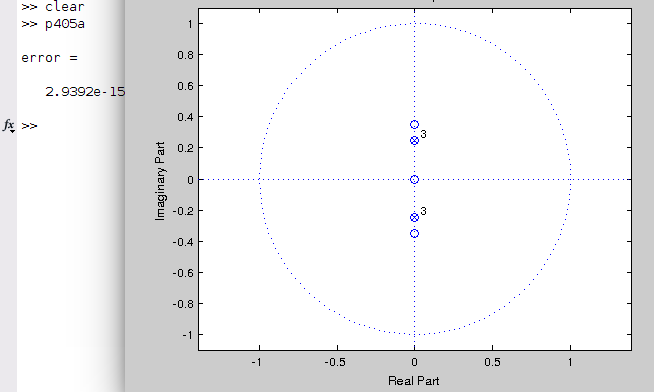
\includegraphics[width=0.5\textwidth,height=0.25\textwidth]{./images/p405-1.png}
	\caption{Problem 4.5-1 Result}
	\label{fig:Problem 4.5-1 Result}
\end{figure}

\section{4.5-2: }


z-transform:
\begin {equation}
\begin {split}
X(z)= 3\frac{1-[0.75cos(0.3\pi)]z^{-1}}{1-2[0.75cos(0.3\pi)]z^{-1}+(0.75)^2z^{-2}} + 4\frac{[0.75sin(0.3\pi)]z^{-1}}{1-2[0.75cos(0.3\pi)]z^{-1}+(0.75)^2z^{-2}}  &\\
= \frac{3+1.1045z^{-1}}{1-0.8817z^{-1} + 0.5625z^{-2}}, |z| > 0.75
\end{split}
\end {equation}


\begin{lstlisting}[style=termstyle]
b = [3 (3*sin(0.3*pi)-2.25*cos(0.3*pi))]; a = [1 -1.5*cos(0.3*pi) 0.5625];
[delta,n1] = impseq(0,0,7); xb1 = filter(b,a,delta); [u,n2] = stepseq(0,0, 7);
xb2 = 3*(((0.75).^n2).*cos(0.3*pi*n2)).*u+4*(((0.75).^n2).*sin(0.3*pi*n2)).*u;
error = max(abs(xb1-xb2))
Hf_1 = figure; set(Hf_1,'NumberTitle','off','Name','P0403b');
[Hz,Hp,Hl] = zplane(b,a); set(Hz,'linewidth',1); set(Hp,'linewidth',1);
title('Pole-Zero plot');
\end{lstlisting}

\begin{figure}[h!]
	\centering
	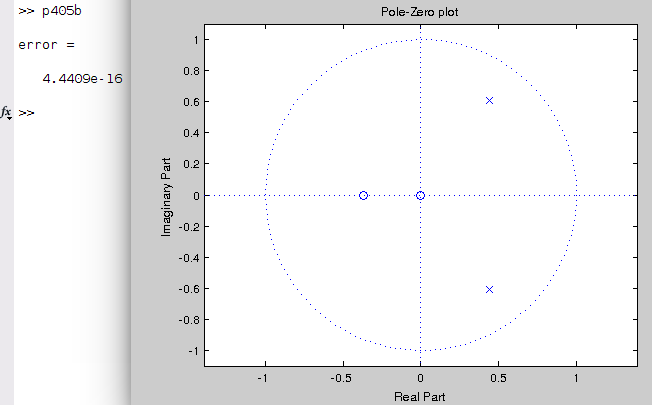
\includegraphics[width=0.5\textwidth,height=0.25\textwidth]{./images/p405-2.png}
	\caption{Problem 4.5-2 Result}
	\label{fig:Problem 4.5-2 Result}
\end{figure}

\section{4.5-3: }

z-transform:
\begin {equation}
\begin {split}
X(z)= \frac{0.866z^{-1}+0.0306z^{-2}-2.486z^{-3}+3.2094z^{-4}-1.62z^{-5}+0.81z^{-6}}{1-2.9z^{-1}+4.8z^{-2}-4.7z^{-3}+2.8z^{-4}-0.9z^{-5}}, |z|>1
\end{split}
\end {equation}

\begin{lstlisting}[style=termstyle]
b = [0 sin(pi/3) (0.81-0.9*sin(pi/3)) -(1.62+sin(pi/3)) (0.9*sin(pi/3)+2.43) -1.62 0.81];
a = [1 -2.9 4.8 -4.7 2.8 -0.9]; [delta,n1] = impseq(0,0,9);
xb1 = filter(b,a,delta);
[u2,n2] = stepseq(0,0,9); [u3,n3] = stepseq(2,0,9);
xb2 = (n2.*sin(pi/3*n2)).*u2+((0.9).^n3).*u3; 

error = max(abs(xb1-xb2))

[Hz,Hp,Hl] = zplane(b,a); set(Hz,'linewidth',1); set(Hp,'linewidth',1);
title('Pole-Zero plot');
\end{lstlisting}

\begin{figure}[h!]
	\centering
	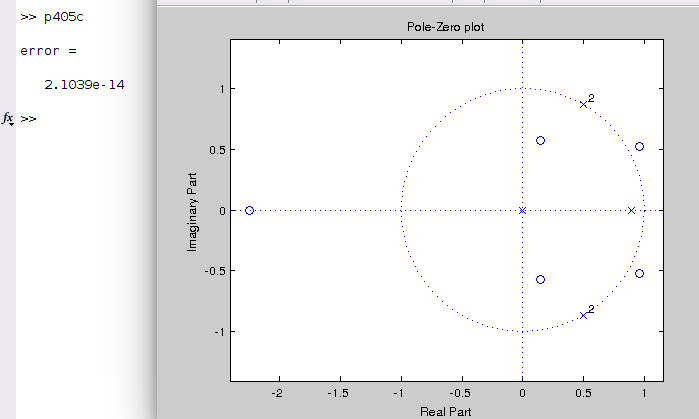
\includegraphics[width=0.5\textwidth,height=0.25\textwidth]{./images/p405-3.png}
	\caption{Problem 4.5-3 Result}
	\label{fig:Problem 4.5-3 Result}
\end{figure}

\section{4.5-4: }

z-transform:
\begin {equation}
\begin {split}
X(z)= \frac{\frac{3}{2}z^{-1}-\frac{2}{3}z^{-3}}{1-\frac{8}{3}z^{-1}+\frac{8}{3}z^{-2}-\frac{32}{27}z^{-3}+\frac{16}{81}z^{-4}}, |z| > \frac{2}{3}
\end{split}
\end {equation}

\begin{lstlisting}[style=termstyle]
b = 3/2*[0 1 0 -4/9]; a = [1 -8/3 8/3 -32/27 16/81];
[delta,n1] = impseq(0,0,8); xb1 = filter(b,a,delta);
[u,n2] = stepseq(1,0,8); xb2 = ((n2.^2).*((2/3).^(n2-2))).*u;
error = max(abs(xb1-xb2))
[Hz,Hp,Hl] = zplane(b,a); set(Hz,'linewidth',1); set(Hp,'linewidth',1);
title('Pole-Zero plot');
\end{lstlisting}

\begin{figure}[h!]
	\centering
	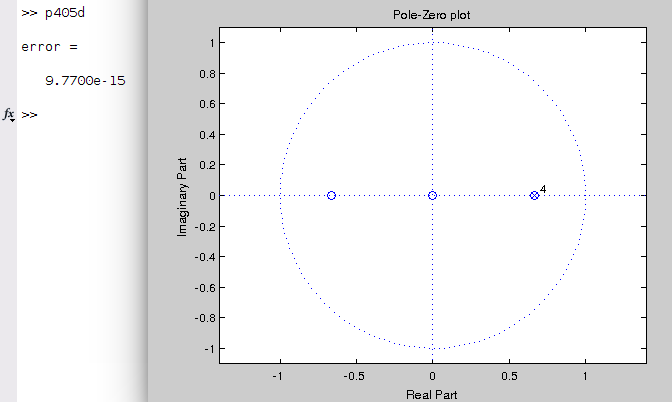
\includegraphics[width=0.5\textwidth,height=0.25\textwidth]{./images/p405-4.png}
	\caption{Problem 4.5-4 Result}
	\label{fig:Problem 4.5-4 Result}
\end{figure}

\clearpage

\section{4.5-5: }

z-transform:
\begin {equation}
\begin {split}
X(z)= \frac{-8z^{-1}-\frac{3}{2}z^{-3}-\frac{1}{16}z^{-5}}{1+\frac{3}{16}z^{-2}+\frac{3}{256}z^{-4}+\frac{1}{4096}z^{-6}}, |z| > \frac{1}{4} 
\end{split}
\end {equation}

\begin{lstlisting}[style=termstyle]
b = [0 -8 0 -1.5 0 -1/16]; a = [1 0 3/16 0 3/256 0 1/(256*16)];
[delta,n1] = impseq(0,0,9); xb1 = filter(b,a,delta);
[u,n2] = stepseq(0,0,9);
xb2 = (((n2-3).*((1/4).^(n2-2))).*cos((pi/2)*(n2-1))).*u;
error = max(abs(xb1-xb2))
[Hz,Hp,Hl] = zplane(b,a); 
set(Hz,'linewidth',1); set(Hp,'linewidth',1);
title('Pole-Zero plot');
\end{lstlisting}

\begin{figure}[h!]
	\centering
	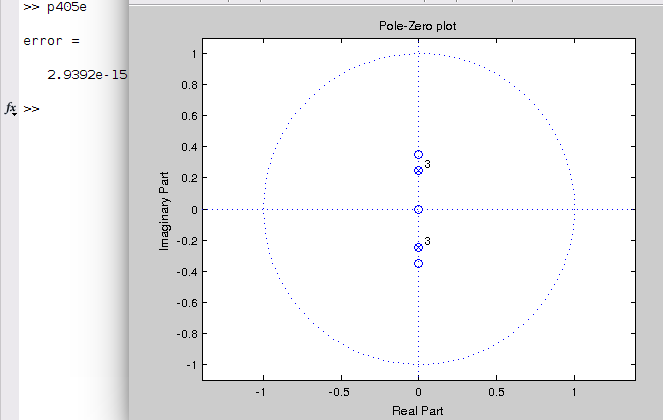
\includegraphics[width=0.5\textwidth,height=0.25\textwidth]{./images/p405-5.png}
	\caption{Problem 4.5-5 Result}
	\label{fig:Problem 4.5-5 Result}
\end{figure}
\end{document}

